We optimize the tree data representation and runtime schedule for MIMD evaluation. We did not see significant parallel speedups when either one was left out. Through a non-trivial amount of experimentation, we found an almost satisfactory combination of existing techniques. It includes popular ideas such as work stealing~[[CITE]] for load-balanced runtime scheduling and tiling~[[CITE]] for data locality, so we report on how to combine them. However, we did not see more than 2X speedups until we added a novel technique to optimize for low  run-time scheduling overheads and temporal data locality: semi-static work stealing. The remainder of this section explores our basic data representation and runtime scheduling techniques.


\begin{figure}
\centering
\subfloat[Na\"{i}ve pointer-based tree representation]{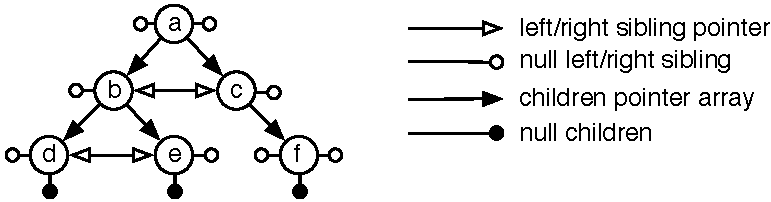
\includegraphics[width=0.6\columnwidth]{chapter6/treenaive}\label{subfig:pointer}} \linebreak
\subfloat[Compressed tree encoding]{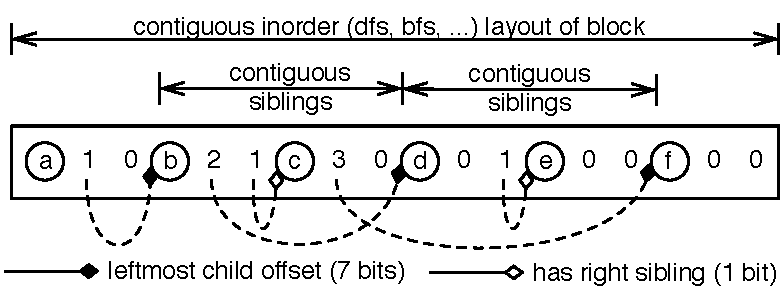
\includegraphics[width=0.6\columnwidth]{chapter6/treecompressed}\label{subfig:compressed}}
\caption{Two representations of the same tree: na\i{v}e pointer-based and optimized. The optimized version employs packing, breadth-first layout, and pointer compression via relative indexing.}
\label{fig:compression}
\end{figure}


\subsection{Data representation: Tuned and Compressed Tiles}

Our data representation optimizes for spatial and temporal locality and, as will be used by the scheduler, low overheads for operating over multiple nodes. Many researchers have proposed individual techniques for similar needs, and it is unclear which to use for what hardware. For example, mobile devices typically have smaller caches than laptops, they should exchange time for space. Our solution was to implement many techniques and build an autotuner~[[CITE]] that automatically choose an effective combination.  

Our autotuner runs sample data on multiple configurations for a particular platform to decide which configuration to use. The most prominent options are:

\begin{itemize}
\item C++ collections or contiguous arrays
\item tiling~\cite{tiling} of subtrees
\item depth-first or breadth-first ordering of nodes in a tile (with matching traversal order~\cite{Chilimbi:1999})
\item aligned data, or unaligned but more packed data
\item pointer compression
\end{itemize}
Several of the techniques are parameterized, so our tuner performs a brute force search for parameter values such as the maximum size of a subtree tile. To make the search tractable, we prune by manually providing heuristics, such as for parameter ranges.

The individual optimizations target several objectives:

\begin{itemize}
\item \textbf{Compression} Compressing the tree better utilizes memory bandwidth and decreases the working set size. We use two basic techniques: structure packing and pointer compression. Packing combines several fields in the same word of memory, such as storing 32 boolean attributes in one 32bit integer field. Similar to \citeauthor{compression}~\cite{compression}, compression encodes node references as relative offsets (16--20bits) rather than 32bit of 64bit pointers. Likewise,  as there are typically few siblings, instead of a counter of number of children (or siblings), we use an \code{isLastSibling} bit. Figure~\ref{fig:compression} depicts a tree using pointers and one of our representations: in the example, the compressed form uses 96\% fewer bits on a 64-bit architecture.

\item \textbf{Temporal and Spatial Locality}  The above compression optimizations improve locality by decreasing the distance between data. To further improve locality, we support rearranging the data in several ways .

Tiling~\cite{tiling} cuts the tree into subtrees and collocates nodes of the same subtree. It improves spatial locality because a node only reads and writes to its neighbors. Likewise, we support breadth-first and depth-first node orderings within a subtree (and across subtrees). Such a representation matches the tree traversal order~\cite{Chilimbi:19999} and therefore improves temporal locality. 

\item \textbf{Prefetching} We supports several options for prefetching to avoid waiting on data reads.  First,  the data access patterns with the data layout, so hardware prefetchers might automatically predict and prefetch data. Second, our compiler can automatically insert explicit prefetch instructions as part of the traversal. Finally, runahead processing~\cite{runaheadprocessing} pre-executes data access instructions. A helper thread traverses a subtree ahead of a corresponding evaluator thread, requesting node data while the evaluator is still computing an earlier thread. We only saw benefits of the first in practice, but leave the others as tunable.


\item \textbf{Parallel scheduling.} Reasoning about individual nodes, such as for load balancing and synchronization, leads to high overheads. By scheduling tiles rather than nodes, we cut overheads. Nodes correspond to tasks in our system, so our approach is a form of \emph{coarsening}. Furthermore, different synchronization strategies are possible for tiles, such as whether to use spin locks, so we autotune over the implementation options. 

We also support several scheduling options. First, we support third-party task schedulers, including Intel TBB~[[CITE]], Cilk~[[CITE]], and those of TesselationOS~[[CITE]]. Second, we built our own that uses a variant of work-stealing threads pinned to processors. It includes options such as whether to use hyper threads or not, and as we saw low speedups when using multiple sockets, how many threads to  use. Our autotuner picks between scheduler implementations.

\end{itemize}

Figure~\ref{fig:compression} depicts several of the data representation optimizations: packing, pointer compression, and a breadth-first layout. 





\subsection{Scheduling: Semi-static Work Stealing}
\subsection{Evaluation}
